% Method figure. Source: figures/src/method.tex (self-contained TikZ; build with `tectonic --outdir .. method.tex` in figures/src).
\begin{figure*}[t]
  \centering
  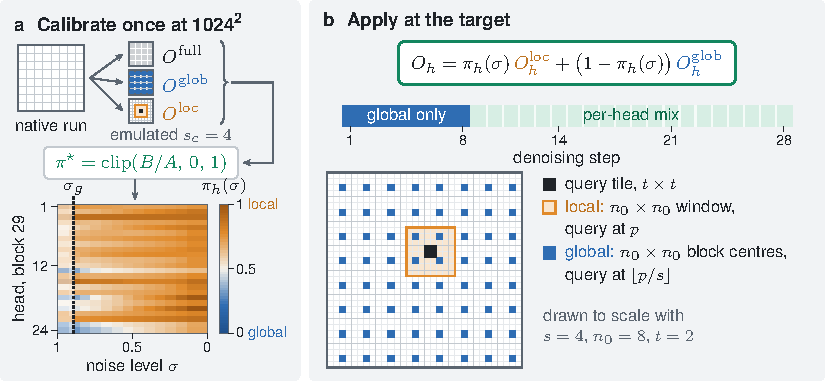
\includegraphics[width=\linewidth]{figures/method.pdf}
  \caption{\textbf{\sca{} mixes a native-size local window with block-centre global keys.} The opening steps, $\sigma>\sigma_g$, use the global operator alone, since high-noise windows repeat structure. Afterwards each head weights the local output by $\pi$, fitted once at $1024^2$ by matching full attention (right: one block's 24 heads by 14 noise bins).}
  \label{fig:method}
\end{figure*}
